\documentclass[11pt]{amsbook}

\usepackage{../HBSuerDemir}

\begin{document}
\hPage{b2p1/242}
\[
	V_r = \frac{dr}{dt} = r
\]
\[
	V_\theta = \frac{V_\theta}{V_r}V_r = (\tan_{\psi})V_r = \frac{r}{dr/d\theta} \cdot \frac{dr}{dt} = \omega r
\]

\[
	V_x = \frac{d}{dt} (r \cos{\theta}) = r \cos{\theta} - (r \sin{\theta})\theta = r \cos{\theta} - \omega r \sin{\theta}
\]
\[
	V_y = \frac{d}{dt}(r \sin{\theta}) = r \sin{\theta} + (r \cos{\theta})\theta = r \sin{\theta} + \omega r \cos{\theta} 
\]


\[
	a_x = \frac{d}{dt} (r \cos{\theta} - \omega r \sin{\theta})
\]
\[
	       = r \cos{\theta} - (r \sin{\theta}  \omega - \omega r \sin{\theta} - (\omega r \sin{\theta}) - (\omega r \cos{\theta})\omega	      
\]
\[
	       = r \cos{\theta} - 2 \omega r \sin{\theta} - \omega r \sin{\theta} - \omega^2r \cos{\theta}
\]
\[
	        r \sin{\theta} + 2 \omega r \cos{\theta} + \omega r \cos{\theta} - \omega^2r \sin{\theta}
\]

or

\[
	a_x = (r - \omega^2r)\cos{\theta} - (2\omega r + \omega r)\sin{\theta}
\]
\[
	a_y = (r - \omega^2r)\sin{\theta} + (2\omega r + \omega r)\cos{\theta}
\]

\[
	a_r = r - \omega^2
\]
$\Rightarrow$ \centerline{(by a rotation)}
\[
	a_\theta = 2\omega r + \omega r
\]

\begin{figure}[h]
\begin{center}
	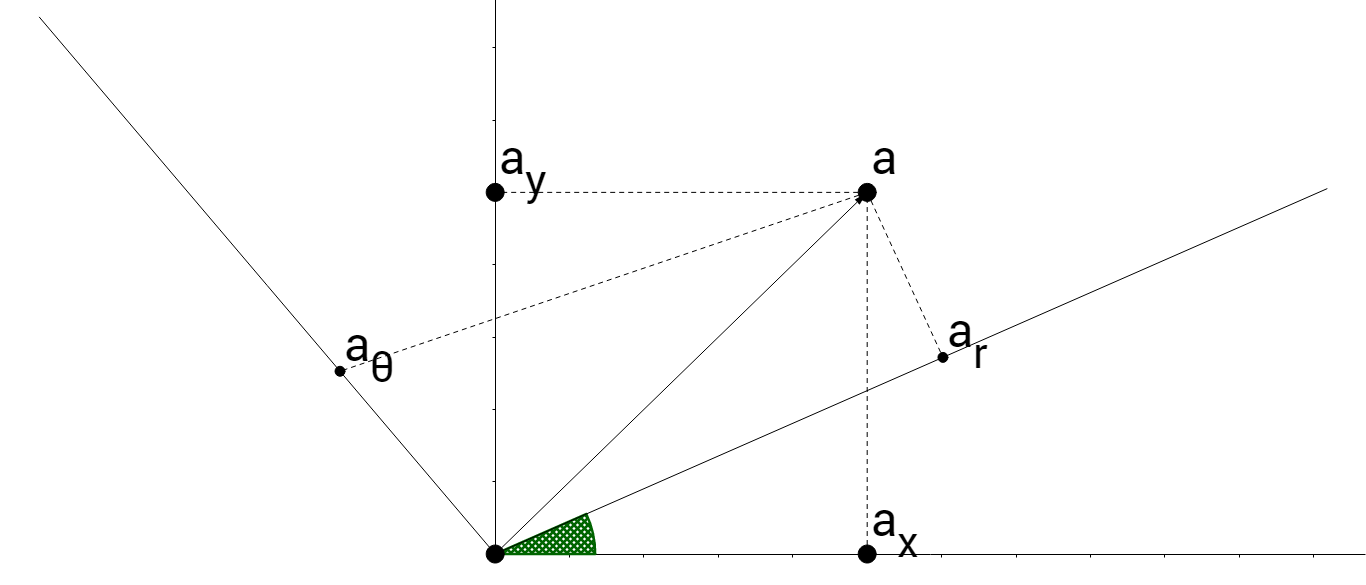
\includegraphics[width=0.50\columnwidth] {images/b2p1-242-fig01.png}
\end{center}
\end{figure}
where $a_r$, $a_{\theta}$ are the radial and transverse components of the acceleration. The motion under a central force (as in planetary motion) the transverse component of the accelaration is zero. We have 
\[
a_{\theta} = 2\omega r + \omega r = \frac{1}{r} (2\omega rr + \omega r^2) = \frac{1}{r} \frac{d}{dt} (\omega r^2)
\]
\[
= \frac{1}{r} \frac{d}{dt} \frac{r^2d\theta}{dt} = \frac{1}{r} \frac{d}{dt} (\frac{d{R_{\Theta r}}}{dt}) = 0 \text{, (for central force)}
\]
\[
\Rightarrow \frac{d{R_\Theta r}}{dt} = const.
\]
\underline{(KEPLER's second law:} The area swept by the radius vector is proportional to time.)

\end{document}